\let\negmedspace\undefined
\let\negthickspace\undefined
\documentclass[journal]{IEEEtran}
\usepackage[a5paper, margin=10mm, onecolumn]{geometry}
\usepackage{lmodern} 
\usepackage{tfrupee} 
\setlength{\headheight}{1cm}
\setlength{\headsep}{0mm}   

\usepackage{gvv-book}
\usepackage{gvv}
\usepackage{cite}
\usepackage{amsmath,amssymb,amsfonts,amsthm}
\usepackage{algorithmic}
\usepackage{graphicx}
\usepackage{textcomp}
\usepackage{xcolor}
\usepackage{txfonts}
\usepackage{listings}
\usepackage{enumitem}
\usepackage{mathtools}
\usepackage{gensymb}
\usepackage{comment}
\usepackage[breaklinks=true]{hyperref}
\usepackage{tkz-euclide} 
\usepackage{listings}                             
\def\inputGnumericTable{}                                 
\usepackage[latin1]{inputenc}                                
\usepackage{color}                                            
\usepackage{array}                                            
\usepackage{longtable}                                       
\usepackage{calc}                                             
\usepackage{multirow}                                         
\usepackage{hhline}                                           
\usepackage{ifthen}                                           
\usepackage{lscape}
\usepackage{xparse}

\bibliographystyle{IEEEtran}

\title{2.9.10}
\author{EE25BTECH11059 - Vaishnavi Ramkrishna Anantheertha}

\begin{document}
\maketitle

\renewcommand{\thefigure}{\theenumi}
\renewcommand{\thetable}{\theenumi}

\numberwithin{equation}{enumi}
\numberwithin{figure}{enumi} 

\textbf{Question}:
Let $\vec a$ and $\vec b$ be two vectors such that
$
\Vert \vec {a} + \vec {b}\rVert = \lVert \vec {b}\rVert.
$
Prove that $\vec a + 2\vec b$ is perpendicular to $\vec a$.
\\
\textbf{Solution: }\\
\begin{table}[H]    
  \centering
  \begin{tabular}{|c|c|}
\hline
\textbf{Name} & \textbf{Value} \\ \hline
$\vec{A}$ & $\myvec{2 & 1 \\0 & 3}$ \\ \hline
\end{tabular}

  \caption{Variables Used}
  \label{tab:2.9.10}
\end{table}

\begin{align}
(\vec {a} + \vec {b})^T(\vec {a} + \vec {b}) = \vec {b}^T \vec {b}.
\end{align}
\begin{align}
(\vec {a} + \vec {b})^T(\vec {a} + \vec {b})
= \vec {a^T} \vec {a} + \vec {a^T} \vec {b} + \vec {b^T} \vec {a} + \vec {b^T} \vec {b}.
\end{align}
Since dot product is symmetric\\
\begin{align}
\vec {a^T} \vec {b} = \vec {b^T} \vec {a}
\end{align}

\begin{align}
\vec {a^T} \vec {a} + 2\,\vec {a^T} \vec {b} + \vec {b^T} \vec {b} = \vec {b^T} \vec {b}.\\
\vec {a^T} \vec {a} + 2\,\vec {a^T} \vec {b} = 0.
\end{align}
We want to show $(\vec {a} + 2\vec {b})$ is perpendicular to $\vec {a}$.\\
\begin{align}
 \text{To prove: }\vec {a^T}(\vec {a} + 2\vec {b}) = 0\\
\vec {a^T}(\vec {a} + 2\vec {b}) = \vec {a^T} \vec {a} + 2\,\vec {a^T} \vec {b}
\end{align}
\\
By eq (0.5) and (0.7)
\begin{align}
\vec {a^T}(\vec {a} + 2\vec {b}) = 0
\end{align}
Hence proved 
\newpage
Refer to Figure

\begin{figure}[H]
\begin{center}
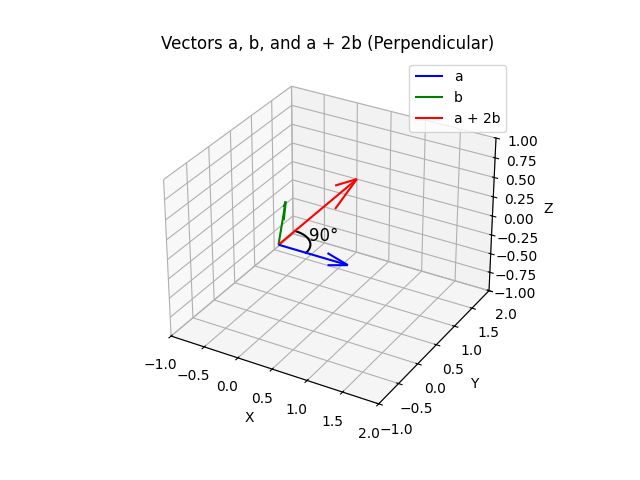
\includegraphics[width=0.6\columnwidth]{figs/graph4.png}
\end{center}
\caption{}
\label{fig:Fig}
\end{figure}
\end{document}  